\subsection*{Teil B: Lineare Funktionen (35 Minuten)}

\begin{enumerate}[label=\arabic*.,resume]

    \item \textbf{Steigung und y-Achsenabschnitt:}

    Bestimme Steigung $m$ und y-Achsenabschnitt $t$ aus der Funktionsgleichung:

    \textit{Beispiel:} $f(x) = 3x + 5$ \hspace{2cm} $m = 3$, $t = 5$

    \vspace{0.5cm}
    \begin{enumerate}[label=\alph*)]
        \item $f(x) = 2x + 7$ \hspace{3cm} $m = $ \underline{\hspace{2cm}}, $t = $ \underline{\hspace{2cm}}

        \item $f(x) = -3x + 1$ \hspace{3cm} $m = $ \underline{\hspace{2cm}}, $t = $ \underline{\hspace{2cm}}

        \item $f(x) = 0,5x - 4$ \hspace{3cm} $m = $ \underline{\hspace{2cm}}, $t = $ \underline{\hspace{2cm}}

        \item $f(x) = -x + 6$ \hspace{3cm} $m = $ \underline{\hspace{2cm}}, $t = $ \underline{\hspace{2cm}}
    \end{enumerate}

    \vspace{1cm}

    \item \textbf{Funktionsgleichung aus Graph ablesen:}

    \begin{center}
        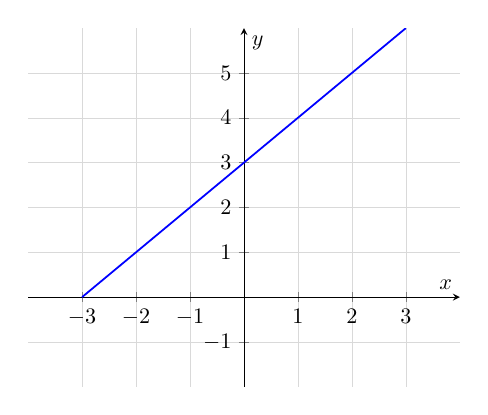
\begin{tikzpicture}[scale=0.8]
            \begin{axis}[
                axis lines = center,
                xlabel = $x$,
                ylabel = $y$,
                xmin=-4, xmax=4,
                ymin=-2, ymax=6,
                xtick={-3,-2,-1,0,1,2,3},
                ytick={-1,0,1,2,3,4,5},
                grid=major,
                grid style={line width=0.1pt,draw=gray!30},
            ]
            \addplot[thick, blue] coordinates {(-3,0) (-2,1) (-1,2) (0,3) (1,4) (2,5) (3,6)};
            \end{axis}
        \end{tikzpicture}
    \end{center}

    Funktionsgleichung: $f(x) = $ \underline{\hspace{6cm}}

    \vspace{0.5cm}

    \item \textbf{Graph zeichnen:}

    Zeichne den Graphen von $f(x) = -2x + 4$ ins Koordinatensystem:

    \begin{center}
        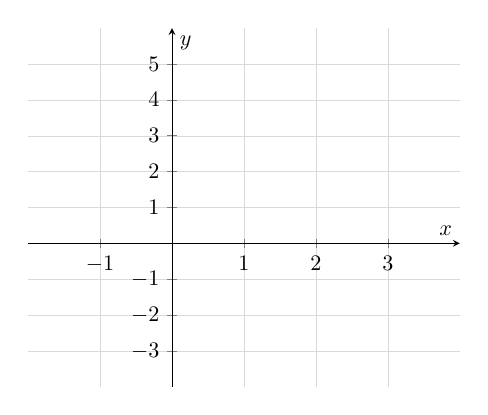
\begin{tikzpicture}[scale=0.8]
            \begin{axis}[
                axis lines = center,
                xlabel = $x$,
                ylabel = $y$,
                xmin=-2, xmax=4,
                ymin=-4, ymax=6,
                xtick={-1,0,1,2,3},
                ytick={-3,-2,-1,0,1,2,3,4,5},
                grid=major,
                grid style={line width=0.1pt,draw=gray!30},
            ]
            \end{axis}
        \end{tikzpicture}
    \end{center}

    \vspace{1cm}

    \item \textbf{Nullstelle berechnen:}

    Berechne die Nullstelle von $f(x) = 3x - 12$

    \textit{Ansatz:} $f(x) = 0$ setzen

    \vspace{2cm}

    Die Nullstelle liegt bei $x = $ \underline{\hspace{4cm}}

\end{enumerate}